\documentclass{article}
\usepackage[spanish, es-tabla]{babel}
\usepackage[utf8]{inputenc}
\usepackage{minted}
\usepackage{amsmath}
\usepackage{geometry}
\usepackage{graphicx}
\usepackage{tabularx}
\usepackage{array}
\usepackage{colortbl}
\usepackage{booktabs}
\usepackage{multirow}
\usepackage{subcaption}
\usepackage{tabularx}

% \geometry{verbose,tmargin=3cm,bmargin=3cm,lmargin=3cm,rmargin=10cm}
% \newcolumntype{Y}{>{\centering\arraybackslash}X}

\newenvironment{exampletwoup}
  {\VerbatimEnvironment
   \begin{VerbatimOut}{example.out}}
  {\end{VerbatimOut}
   \setlength{\parindent}{0pt}
   \fbox{\begin{tabular}{l|l}
   \begin{minipage}{0.55\linewidth}
     \inputminted[fontsize=\small,resetmargins]{latex}{example.out}
   \end{minipage} &
   \begin{minipage}{0.35\linewidth}
     \input{example.out}
   \end{minipage}
\end{tabular}}}


\begin{document}

\begin{tabular}{||l|l||l|l||l|l||} \hline
  \emph{declaración} & \emph{tamaño} & \emph{declaración} & \emph{tamaño} & \emph{declaración} & \emph{tamaño} \\ \hline
  \texttt{\{\textbackslash tiny ...\}} & \tiny size & \texttt{\{\textbackslash normalsize ...\}} & \normalsize size & & \\
  \texttt{\{\textbackslash scriptsize ...\}} & \scriptsize size & \texttt{\{\textbackslash large ...\}} & \large size & & \\
  \texttt{\{\textbackslash footnotesize ...\}} & \footnotesize size & \texttt{\{\textbackslash Large ...\}} & \Large size & \texttt{\{\textbackslash huge ...\}} & \huge size\\
  \texttt{\{\textbackslash small ...\}} & \small size & \texttt{\{\textbackslash LARGE ...\}} & \LARGE size & \texttt{\{\textbackslash Huge ...\}} & \Huge size \\ \hline
\end{tabular}


% Test 
% \begin{table}
%   \centering
% 	\begin{subtable}[b]{0.45\textwidth}
% 		\centering
% 		\resizebox{0.9\textwidth}{!}{\begin{tabular}{|c|c|c|c|c|} \hline
% 			       & \multicolumn{4}{c|}{Calificaciones}                                      \\ \hline
% 			Nombre & Parcial 1                           & Parcial 2 & Parcial 3 & Definitiva \\ \hline
% 			Pedro  & 4.5                                 & 4.6       & 4.8       & 4.6        \\
% 			Alicia & 5.0                                 & 4.8       & 5.0       & 4.9        \\
% 			Johana & 3.4                                 & 2.8       & 2.9       & 3.0        \\ \hline
% 		\end{tabular}}
% 		% \caption{\label{tab:notas} Estas son las notas de Física: Mecánica}
% 		\caption{Tabla a}
%   \end{subtable}%
% 	\begin{subtable}[b]{0.45\textwidth}
% 		\centering
% 		\resizebox{0.9\textwidth}{!}{\begin{tabular}{|c|c|c|c|c|} \hline
% 			       & \multicolumn{4}{c|}{Calificaciones}                                      \\ \hline
% 			Nombre & Parcial 1                           & Parcial 2 & Parcial 3 & Definitiva \\ \hline
% 			Pedro  & 4.5                                 & 4.6       & 4.8       & 4.6        \\
% 			Alicia & 5.0                                 & 4.8       & 5.0       & 4.9        \\
% 			Johana & 3.4                                 & 2.8       & 2.9       & 3.0        \\ \hline
% 		\end{tabular}}
% 		% \caption{\label{tab:notas} Estas son las notas de Física: Mecánica}
% 		\caption{Tabla b}
% 	\end{subtable}
% 	\caption{Dos subtablas}
% \end{table}

% Test
% \begin{figure}
%   \centering
%   \begin{subfigure}[b]{0.35\textwidth}
%     \centering
%     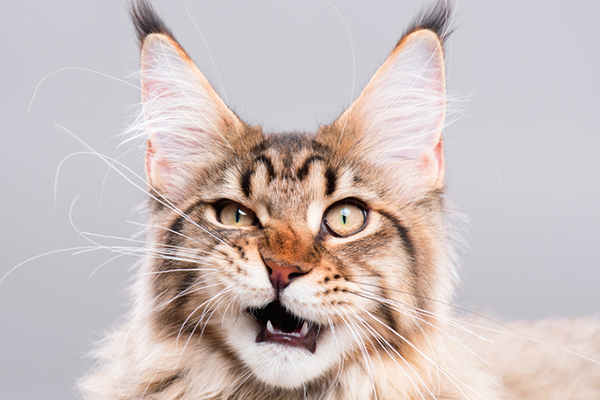
\includegraphics[width=\linewidth]{gato}
%     \caption{Gato}\label{fig:gato}
%   \end{subfigure}%
%   \begin{subfigure}[b]{0.35\textwidth}
%     \centering
%     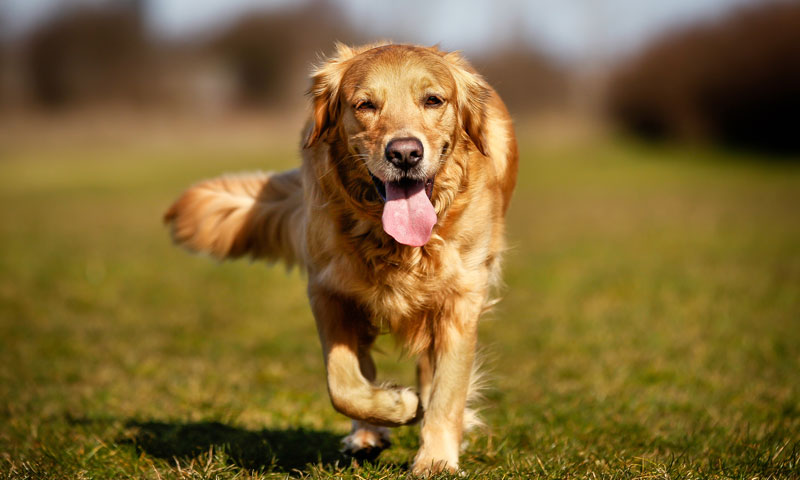
\includegraphics[width=\linewidth]{perro}
%     \caption{Perro}\label{fig:perro}
%   \end{subfigure} \\ 
%   \begin{subfigure}[b]{0.35\textwidth}
%     \centering
%     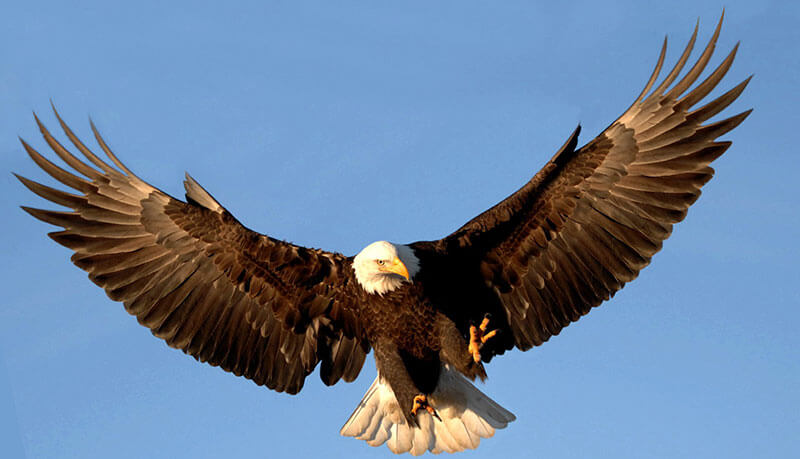
\includegraphics[width=\linewidth]{aguila}
%     \caption{Águila}\label{fig:aguila}
%   \end{subfigure}

%   \caption{Mascotas}\label{fig:mascotas}
% \end{figure}


\end{document}